\chapter{Neighbourhood component analysis}
\label{ch:nca}

	Neighbourhood Component Analysis (NCA; \citealp{goldberger2004}) learns a Mahalanobis metric that improves the performance of $k$ nearest neighbours ($k$NN). From a practical point of view, NCA  is regarded as a desirable additional step before doing classification with $k$NN. It improves the classification accuracy and it is also provides good low-dimensional representation of the data.

\section{General presentation}
\label{sec:general-presentation}

	Because the goal is to enhance the $k$NN performance, the first idea \citet{goldberger2004}
	had was to maximize the leave one out cross validation performance with respect to a linear projection $\AB$. The procedure can be described as follows: apply the linear transformation $\AB$ to the whole data set, then take each 
	point $\AB\xB_i$ and classify it using $k$NN on the transformed data set $\{\AB\xB_j\}_{j=1}^N$. The matrix $\AB$ that achieves the highest number of correct classifications will be used for testing. Unfortunately, any objective function based on the $k$ nearest neighbours
	is piecewise constant and discontinuous and, hence, hard to optimize. The reason is that there does
	not exist an exact correlation between $\AB$ and the neighbours
	of a given point: a small perturbation in $\AB$ might cause strong changes or, conversely, 
	it might leave the neighbours unchanged.
	
	The authors' solution lies in the concept of \textit{stochastic} nearest
	neighbours. Remember that in the classical scenario, a query point gets the label of the closest point. In the stochastic nearest neighbour 
	case, the query point inherits the label of a neighbour with a probability that is inverse proportional with the distance. The stochastic function is reminiscent of the softmax activation used for neural networks or the generalized logistic function. So $p_{ij}$ is the probability that the point $\xB_j$ is selected as the nearest neighbour of the point $\xB_i$ and it is given by:
	\begin{align}
		p_{ij} = \frac{
						\exp(-d_{ij}^2)
					  }{
						\sum_{\substack{k=1 \\k\neq i}}^N\exp(-d_{ik}^2)
					  },
	\label{eq:stochastic-neighbour}
	\end{align} where $d_{ij} = d(\AB\xB_i;\AB\xB_j) = (\xB_i-\xB_j)\tr\AB\tr\AB(\xB_i-\xB_j)$; also we set $p_{ii}=0$: point~$\xB_i$ cannot pick itself as the nearest neighbour.
	Now we can construct a continuous objective function using the stochastic assignments~$p_{ij}$ which are differentiable with respect to~$\AB$.
	
	A suitable quantity to maximize is the probability of each point of getting correctly classified. A point $\xB_i$ is correctly classified when it is selected by a point $\xB_j$ that has the same label as $\xB_i$:
	\begin{align}
		p_i = \sum_{j\in c_i} p_{ij}.
	\end{align}
	
	The objective function considers each point in the data set and incorporates their probability of belonging to the true class:
	\begin{align}
		f(\AB) &= \sum_{i=1}^N p_i\notag\\
			   &= \sum_{i=1}^N \sum_{j\in c_i} \frac{
								\exp(-d_{ij}^2)
							  }{
								\sum_{k\neq i}\exp(-d_{ik}^2)
							  }.
	\label{eq:nca-obj}
	\end{align}
	The score given by the objective function can be interpreted as the expected number of the correctly classified points.
	
	We maximise $f(\AB)$ using an iterative gradient based solver such as gradient ascent, conjugate gradients or delta-bar-delta, see Subsection \ref{subsec:optimization}. For the optimisation, we need the numerical expression of the gradient. If we differentiate with respect to $\AB$, we obtain:
	\begin{align}
	  \frac{\partial f}{\partial
	\AB}=2\AB\sum_{i=1}^{N}\left(p_i\sum_{k=1}^Np_{ik}\xB_{ik}\xB_{ik}^{\textrm{T}} -
	\sum_{j\in c_i}p_{ij}\xB_{ij}\xB_{ij}^{\textrm{T}} \right)\label{eq:nca-grad},
	\end{align}
	where $\xB_{ij} = \xB_i - \xB_j$. The interested reader can find the derivation of the gradient in the appendix. 
	
	It is useful to note that NCA's objective function is not convex. So care must be taken to avoid poor local optima. The choice of initialization and of the optimization method affect the quality of the final solution. Section \ref{sec:practical-notes} discusses these and other practical issues. On the other hand, the non-convexity property has its advantage. It allows NCA to get good results on more complicated data sets that are not non convex. 

	Another important aspect is the computational cost of the method. For each point, we need to compute all the pairwise distances $d_{ij}$ which has the cost of $\mathcal{O}(dN^2)$. But prior to that, we have to compute the point projections $\{\AB\xB_i\}_{i=1}^N$; this operation is done in $\mathcal{O}(dDN)$ flops. So the total cost of evaluating the objective function $f(\AB)$ is  $\mathcal{O}(dDN+dN^2)$. Chapter \ref{ch:reducing} treats NCA's computational drawback; there are presented different ideas of speeding up the computations.
	
	The general scenario in which NCA is applied can be described by the training and testing steps:
	describe algorithm.
	%\begin{itemize}
	%   \item
	%\end{itemize}
	
\section{Class-conditional kernel density estimation interpretation}
\label{sec:cc-kde}
	
	\begin{figure}
	  \centering
	  \subfigure[Illustration of the class as a mixture of
	Gaussians.]{\label{fig:mog}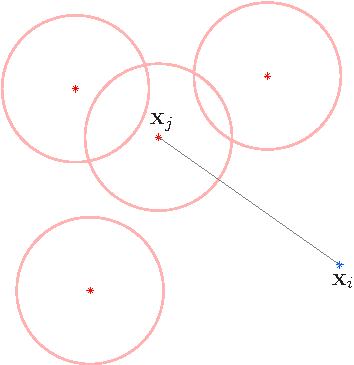
\includegraphics[width=6cm]{images/mog}}
	%\subfigure[The projection $\AB$ applied to the whole data set
	%$\mathcal{D}$.]{\label{fig:sub-sampling-2}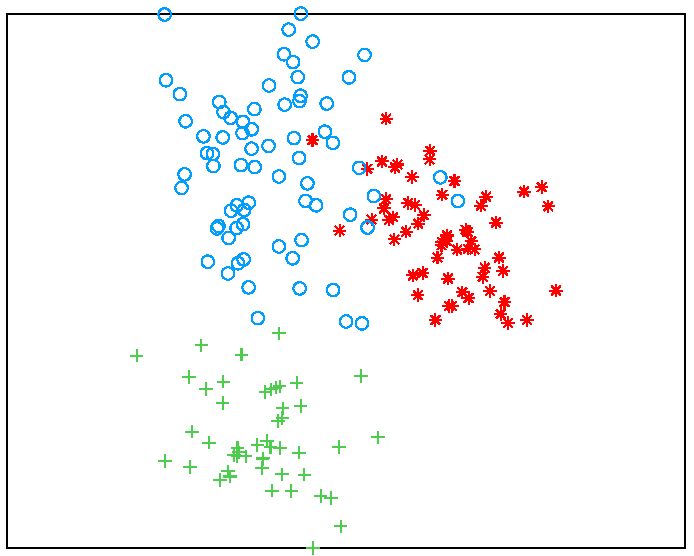
\includegraphics[width=0.48\textwidth]{images/sub-sample-2}}
	  \caption{Formulating NCA as a class-conditional kernel density estimation
	framework.}
	  \label{fig:kde}
	\end{figure}
	
	In this section we will present NCA into a class-conditional kernel density
	estimation framework. This interpretation will allow us to understand what are
	the assumptions behind NCA. Moreover, this also offers the possibility of
	altering the model in a suitable way that is efficient for computations. We will
	see this in the sections \ref{sec:approximate} and \ref{sec:exact-computations}.
	Similar ideas were previously presented by and , but the following were derived
	independently and they offer different insights. The following interpretation
	was inspired by the probabilistic $k$NN presented by \citet{barber2011}.
	
	We start with the basic assumption that each class can be modelled by a mixture
	of Gaussians. For each of the $N_c$ data points in class $c$ we consider a
	Gaussian ``bump'' centred around it. From a generative perspective, we can view
	that each point $\xB_j$ can generate a point $\xB_i$ with a probability given by
	an isotropic normal distribution with variance $\sigma^2$:
	\begin{align}
	    p(\xB_i|\xB_j) &= \mathcal{N}(\xB_i|\xB_j, \sigma^2\mathrm{I}_D) \\
	                   &= \frac{1}{(2\pi)^{D/2}}\exp \left\{-\frac{1}{2\sigma^2}
	(\xB_i - \xB_j)^\mathrm{T}(\xB_i - \xB_j)\right\}.
	\end{align}
	
	By changing the position of the points through a linear transformation $\AB$,
	the probability changes as follows:
	\begin{align}
	    p(\AB\xB_i|\AB\xB_j) \propto \exp \left\{-\frac{1}{2\sigma^2} (\xB_i -
	\xB_j)^\mathrm{T}\AB^\mathrm{T}\AB(\xB_i - \xB_j)\right\}.
	\end{align}
	
	We can note that this is similar to the $p_{ij}$ from NCA. Both
	$p(\AB\xB_i|\AB\xB_j)$ and $p_{ij}$ are directly proportional with the same
	quantity.
	
	Using the mixture of Gaussians assumption, we have that the probability of a
	point of being generated by class $c$ is equal to the sum of all Gaussians in
	class $c$:
	\begin{align}
	    p(\xB_i|c) &= \frac{1}{N_c}\sum_{\xB_j \in c} p(\xB_i|\xB_j)\\
	               &= \frac{1}{N_c}\sum_{\xB_j \in c} \mathcal{N}(\xB_i|\xB_j,
	\mathrm{I}_D).
	\end{align}
	
	However, we are interested on the inverse probability, given a point $\xB_i$
	what is the probability of $\xB_i$ belonging to class $c$. We can obtain an
	expression for $p(c|\xB_i)$ using Bayes' theorem:
	\begin{align}
	    p(c|\xB_i) = \frac{p(\xB_i|c)p(c)}{p(c|\xB_i)} =
	\frac{p(\xB_i|c)p(c)}{\sum_{c} p(\xB_i|c)p(c)}.
	    \label{eq:nca-cc-kde-bayes}
	\end{align}
	
	Now if further consider the classes to be equal probable (which might a
	reasonable assumption if we have no a priori information) we arrive at result
	that resembles the expression of $p_i$ (see equation):
	\begin{align}
	%   &p(c|\xB_i) = \frac{p(\xB_i|c)}{\sum_{c} p(\xB_i|c)}\\
	    p(c|\AB\xB_i) = \frac{
	                \frac{1}{N_c}\sum_{\xB_j \in
	c}\exp\left\{-\frac{1}{2\sigma^2}(\xB_i -
	\xB_j)^\mathrm{T}\AB^\mathrm{T}\AB(\xB_i - \xB_j)\right\}
	                }
	                {
	                \frac{1}{N_{c'}}\sum_{c'} \sum_{\xB_k \in
	c'}\exp\left\{-\frac{1}{2\sigma^2}(\xB_i -
	\xB_k)^\mathrm{T}\AB^\mathrm{T}\AB(\xB_i - \xB_k)\right\}
	                }
	\end{align}
	
	%In the numerator we have the sum of
	We are interested in predicting the correct class of the point $\xB_i$. So we
	try to find that linear transformation $\AB$ that maximises the class
	conditional probability of this point $p(c_i|\xB_i)$ to its true class $c_i$.
	\begin{align}
	    f(\AB) = \sum_i p(c_i|\AB\xB_i).
	    \label{eq:nca-cc-kde-obj}
	\end{align}.
	
	The gradient of the objective function is the following:
	\begin{align}
	    \frac{\partial f}{\partial \AB} =
	      \sum_i \left\{
	                \frac
	                {
	                    \frac{\partial p(\AB\xB_i|c)}{\partial \AB}p(c)
	                }
	                {
	                    \sum_c p(\xB_i|c)p(c)
	                }
	                - \underbrace{\frac{
	                    p(\AB\xB_i|c)p(c)
	                }{
	                    \sum_c p(\AB\xB_i|c)p(c)
	                }}_{p(c|\AB\xB_i)}
	                \frac{
	                    \sum_c \frac{\partial p(\AB\xB_i|c)}{\partial \AB}p(c)
	                }{
	                    \sum_c p(\AB\xB_i|c)p(c)
	                }
	             \right \}.
	    \label{eq:nca-cc-kde-grad}
	\end{align}
	

\section{Practical notes}
\label{sec:practical-notes}

	This section provides some practical advice for the questions 
	that can be raised while implementing NCA. 
	While NCA is not that hard to implement, there is needed certain care
	in order to achieve good solutions.

\subsection{Optimization methods}
\label{subsec:optimization}

	The function $f(\AB)$, equation \ref{eq:nca-obj}, can be maximised using any gradient based optimizer. We considered two popular approaches for our implementation: gradient ascent and conjugate gradients. These are only briefly presented here. The interested reader is pointed to \citet{bishop1995}.

	\subsubsection*{Gradient ascent}

	Gradient ascent is one of the simplest optimisation methods. It is an iterative algorithm that aims to find the maximum of a function by following the gradient direction at each step. The entire procedure is summarized by algorithm \ref{alg:gd}.
      
	\begin{algorithm} 
		\caption{Gradient ascent (batch version)} 
		\label{alg:gd}  
		\begin{algorithmic}[1]                    % enter the algorithmic environment
			\REQUIRE Data set $\mathcal{D}=\{\xB_1,\cdots,\xB_N\}$.
			\STATE{ Get initial $\AB_0$ } \label{alg:gd-init}
			\REPEAT
				\STATE {Update parameter: $\AB_{t+1}\leftarrow \AB_{t} + \eta\frac{\partial
f(\AB_{t},\mathcal{D})}{\partial\AB}$}
				\STATE {Update learning rate $\eta$}
				\STATE {$t\leftarrow t+1$}
			\UNTIL {convergence}
			\RETURN $\AB_{t}$.
		\end{algorithmic}
	\end{algorithm}

	There are three aspects we need to carefully consider:
	\begin{enumerate}
	 \item The algorithm starts the search in the parameter space from the an initial parameter~$\AB_0$. Different values for $\AB_0$ will give different final solutions. In the NCA context, initialization is related to finding a good initial linear transformation; this is discussed  separately in subsection \ref{subsec:initialization}. For the moment, we can assume the values of $\AB_0$ are randomly chosen.
	 \item The parameter $\eta$ is called \textit{step size} or, in neural networks related literature, it also known as \textit{learning rate}. As name suggests, $\eta$ controls how much we move the parameter in the gradient direction. 

	The learning rate can be either fixed or adaptive. For the first case, choosing the correct value for $\eta$ is critical. If $\eta$ is set too large, the algorithm diverges. On the other hand, a small $\eta$ results in slow convergence. 

	Usually, a variable learning rate $\eta$ is preferred since its more flexible. The ``bold driver'' is a heuristic for modifying $\eta$ during training.

% 	A popular choice for an 
	 \item Stopping criterion. 
	\end{enumerate}


% 	The notation $\frac{\partial f(\AB_t,\mathcal{D})}{\partial \AB}$

	\subsubsection*{Conjugate gradients}
	

% \begin{itemize}
%     \item We have the first-order gradient information; so, we
%         can use any gradient based method.
%     \item Gradient descent is an iterative algorithm that uses
%         first-order information to find a minimum of a
%         function. At each step, it proposes to go in the
%         steepest direction, \ie, the direction with largest
%         gradient. It is a very simple to implement method, but
%         suffers from known convergence drawbacks. For example,
%         there might appear the zig-zagging effect it depends
%         on some critical parameters which make it difficult to
%         use in practice. These are the learning rate $\eta$
%         and the convergence conditions.
%     \item Common choices for $\eta$ are either using a
%         constant step or decrease it gradually. Using a
%         constant step size can make the algorithm diverge.
%     \item There are different other heuristics that make this
%         more efficient. One of these is the bold-driver trick.
%     \item A learning rate decreasing procedure is to set
%         $\eta=\frac{\eta_0}{t + t_0}$, where $t$ represents
%         the iteration number, $\eta_0$ and $t_0$ are
%         constants. So, we end up with two hyper-parameters
%         instead of one. There are various trick of tuning
%         them. Leon Bottou mentions that a common value for
%         $\eta_0$ is to be equal to the regularization variable
%         and $t_0$ should then be selected such that the
%         updates . In our implementation, because we did not
%         use a regularization term, we set $\eta_0$ to a fix
%         value and then we did an exponential search for $t_0$.
%     \item One might also try to use momentum. For further
%         useful advice on optimization one should consult
%         BackProp.
%     \item An improved version of the gradient descent is the
%         conjugate gradients algorithm. This has better
%         convergence.
% \end{itemize}

\subsection{Initialization}
\label{subsec:initialization}

    \begin{figure}
	  \centering
	  \subfigure[Initial random projection]{\label{fig:init-1}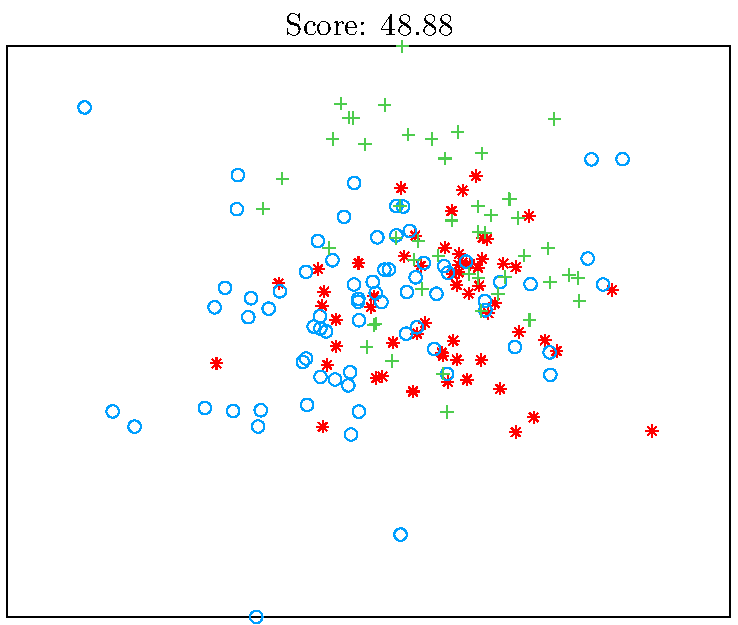
\includegraphics[width=0.49\textwidth]{images/wine-init-1}}
	  \subfigure[NCA projection after random initialization]{\label{fig:init-2}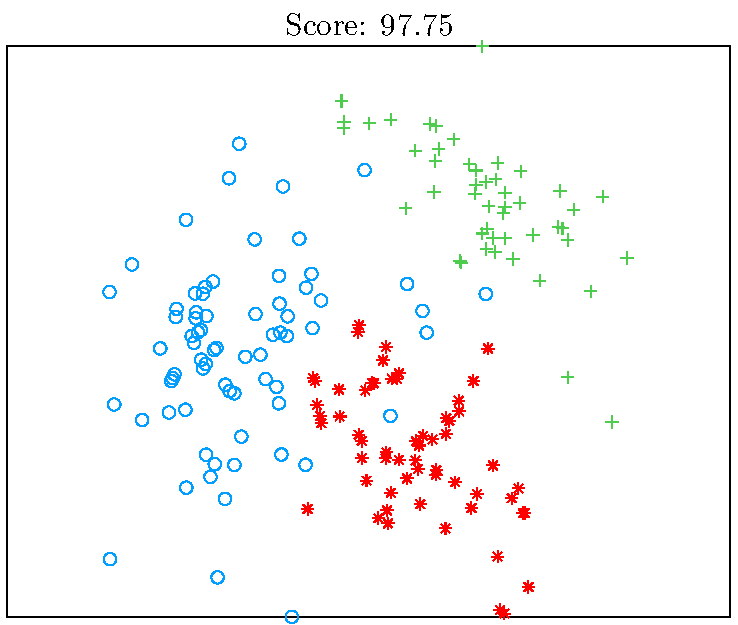
\includegraphics[width=0.49\textwidth]{images/wine-init-2}}

	  
	  \subfigure[Initial projection using PCA]{\label{fig:init-3}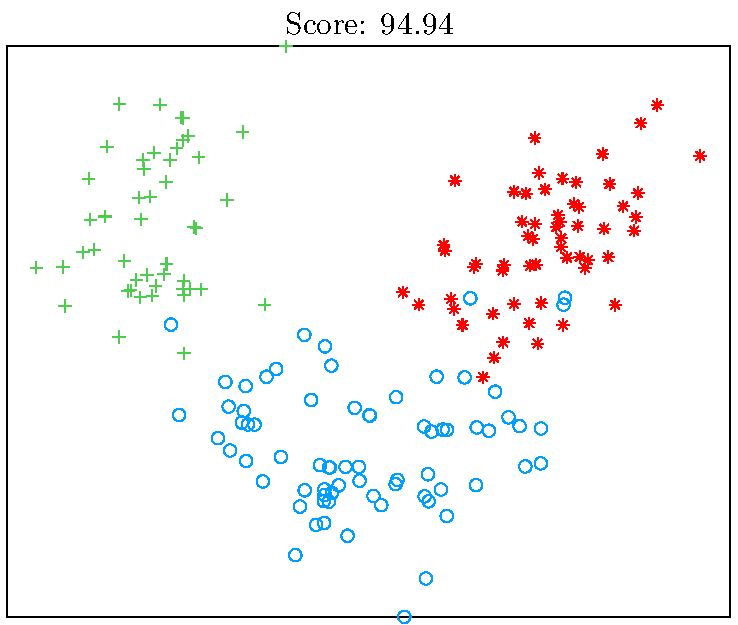
\includegraphics[width=0.49\textwidth]{images/wine-init-3}}
	  \subfigure[NCA projection after PCA initialization]{\label{fig:init-4}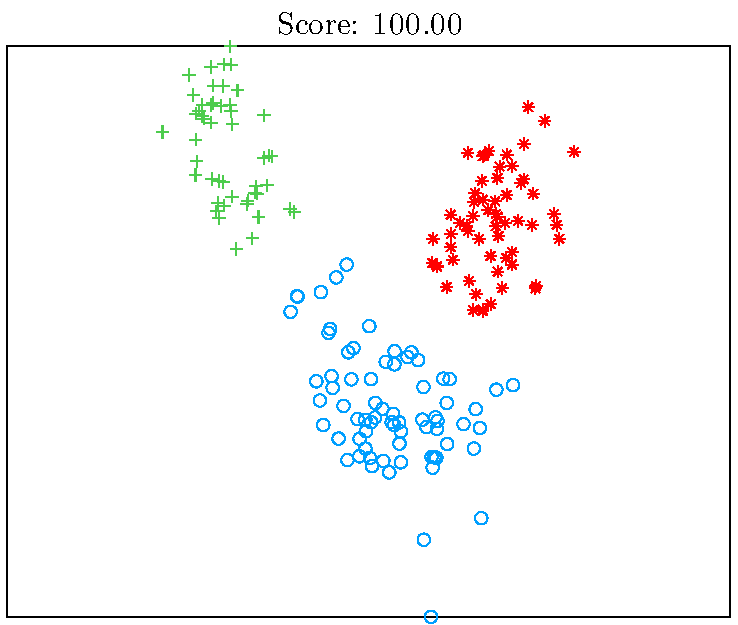
\includegraphics[width=0.49\textwidth]{images/wine-init-4}}

	  
	  \subfigure[Initial projection using LDA]{\label{fig:init-7}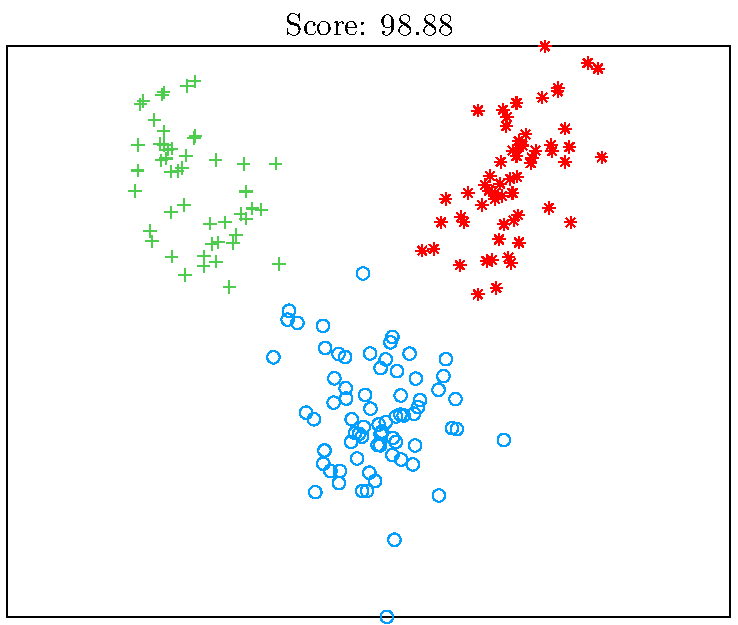
\includegraphics[width=0.49\textwidth]{images/wine-init-5}}
	  \subfigure[NCA projection after LDA initialization]{\label{fig:init-8}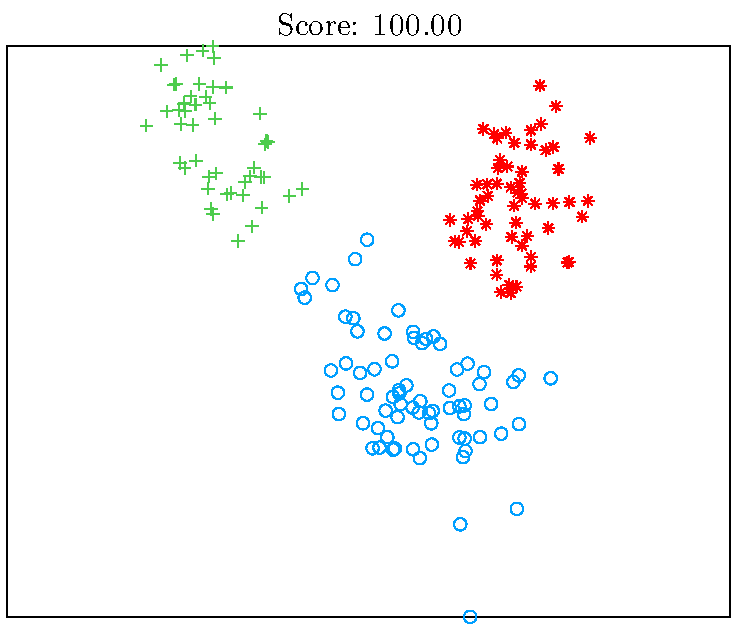
\includegraphics[width=0.49\textwidth]{images/wine-init-6}}
	  
	  \caption{\small Results for different initializations (random, PCA and LDA) on \texttt{wine} data set. The images on the left side represent the projections of the data set using the initial $\AB$. The images on the right side are data set projection with the final $\AB$. Above each figure there is presented the LOOCV score which is normalized to 100.}
	  \label{fig:init}
    \end{figure}

    Initialization is important because the function $f(\AB)$ is not convex. The quality of the final solution relies on the starting point of the optimisation algorithm. A general rule of thumb is to try multiple initial seeds and select that final $\AB$ that gives the highest score.

    We have already mentioned random initialization in subsection \ref{subsec:optimization}. Beside this, we can linear transformations that are cheap to compute. Such examples include  principal component analysis (PCA; \citealp{pearson1901}), linear discriminant analysis (LDA; \citealp{fisher1936}) and relevant component analysis (RCA; \citealp{bar2003}). For completeness, we give here the equations and also include further notes:
        \begin{itemize}
            \item  PCA finds an orthogonal linear
                transformation of the data. This is
                obtained by computing the
                eigendecomposition of the outer covariance
                matrix:
                \begin{align}
                    \SB = \frac{1}{N}\sum_{i=1}^N (\xB-\muB)(\xB-\muB)\tr.
                    \label{eq:pca-1}
                \end{align}

            \item LDA finds a linear transformation $\AB$ by maximizing the
variance between classes $\SB_B$ relative to the amount of within-class variance
$\SB_W$:
            \begin{align}
             \SB_B &=
\frac{1}{C}\sum_{c=1}^{C}\boldsymbol\mu_c\boldsymbol\mu_c\tr\label{eq:lda-1}\\
             \SB_W &= \frac{1}{N}\sum_{c=1}^{C}\sum_{i \in
c}(\mathbf{x}_i-\boldsymbol{\muB}_c)(\mathbf{x}_i-\boldsymbol{\mu}_c)\tr.\label{eq:lda-2}
            \end{align}

            The projection matrix $\AB$ that achieves this maximization consists
of the eigenvectors of $\SB_W^{-1}\SB_B$.

            Unlike PCA, LDA makes use of the class labels and this
usually guarantees a better initial projection.

            \item RCA finds a linear transformation $\AB$
                that ``whitens'' the data with respect to
                the within-chunklet covariance matrix.
                Because for NCA we restrict ourselves to
                fully labelled data, the within-chunklet
                covariance is the within-class covariance
                $\SB_W$, Equation \ref{eq:lda-2}. The
                whitening transformation is then
                $\AB=\SB_W^{-1/2}$.
        \end{itemize}

        If the projection is full-rank, $\AB\in\mathbb{R}^{D\times D}$, other obvious initializations are the identity matrix $\AB=\mathrm{I}_D$ and the Mahalanobis linear transformation $\AB=\SB^{-1/2}$.

	If we want to learn a low-rank projection, $\AB \in \mathbb{R}^{d\times D},d<D$, then we can still use the eigendecomposition based methods. We construct $\AB$ using only the top $d$ most
        discriminative eigenvectors, \ie, those eigenvectors that have the
        highest eigenvalues associated.

        From our experiments, we conclude that a good
        initialization reflects in a good solution and a better convergence; this benefits are more evident
        large data sets. As advertised in , we found RCA to work the best. Figure depicts initialization effects on a small data set.

\subsection{Numerical issues}
\label{subsec:numerical-issues}

	Numerical problems can easily appear when computing the soft assignments $p_i$. If a point
        $\xB_i$ is far away from the rest of the points, the stochastic probabilities $p_{ij}, \forall j,$ are all 0 in numerical precision. Consequently, the result $p_i$ is undetermined: $\frac{0}{0}$. 
	To make an idea of how far $\xB_i$ has to be for this to happen, let us consider an example in \textsc{Matlab}. The answer to 
        \texttt{exp(-d\^{}2)} is \texttt{0} whenever \texttt{d} exceeds \texttt{30} units.
	This is problematic in practice, since distances larger than 30 often appear. Some common cases include data sets that contain outliers or data sets that present a large scale. 

	The large scale effect can be partially alleviated if we initialize $\AB$ with small values. This is idea was used by Laurens van der Maaten in his implementation: \texttt{A = 0.01*randn(d,D)}. However, this does not guarantee to compensate the scale variation for any data set.

% 	projection $\AB$ does not compensate for the scale

	A more robust solution is to normalize the
        data, \ie, centre and making it unit variance:
        \begin{align}
            x_{ij} \leftarrow \frac{x_{ij} - \mu_j}{\sigma_j}, i =
	    \{1,\cdots,N\}, j = \{1,\cdots,D\}.
        \end{align}
        In this case, we have to store the initial mean and variance of the data
        and, at test time, transform the test data accordingly: subtract the mean and scale it using the variance coefficients. The variance scaling can be regarded as a linear transformation. We can combine this transformation with the learnt transformation $\AB$ and get:
        \begin{align}
            \AB_{\text{total}} \leftarrow \AB  \cdot \begin{pmatrix}
                  \sigma_1 &  \cdots & 0 \\
                  \vdots  &   \ddots & \vdots  \\
                  0 & \cdots & \sigma_D
                 \end{pmatrix}.
        \end{align}

	
	In general, data normalization avoids numerical issues for the first iterations. But during training, the scale of $\AB$ increases and data points can be ``thrown'' away. We adopt a rather simplistic approach to avoid any numerical problems: replace $p_i$ with a very small value whenever we are in the $\frac{0}{0}$ case, as in Laurens van der Maaten implementation. In \textsc{Matlab}, this is done using the following command \texttt{max(p\_i,eps)}. 
    
	A more robust more rigorous way of dealing with this by multiplying both the numerator and denominator of $p_i$ with a certain quantity $\exp(L)$:
	\begin{align}
	  p_i = \frac{\sum_{j\in c_i} \exp(L-d_{ij}^2)}{\sum_{k\neq i} \exp(L-d_{ik}^2)},
	\end{align}
	where $L = \min_{k\neq i} d_{ik}^2$. This value of $L$ ensures that at least one term in the denominator does not undeflow.

	In our implementation, we preferred the previous trick because of its simplicity and speed.

\subsection{Regularization}
\label{subsec:regularization}

  Although the original paper \citep{goldberger2004} claimed that there were no problems with overfitting, we observed that NCA objective function has the tendency to increase the scale of the linear projection~$\AB$. \citet{butman2008} pointed out that this is especially problematic for data sets whose size~$N$ is significantly smaller than the dimensionality~$D$. In such a case, the linear transformation~$\AB$ can be chosen to project each point~$\xB_i$ to a pre-specified a location~$\yB_i$. The values of $\AB$ are obtained by solving the linear system:
  \begin{align}
    \AB\xB_i = \yB_i, \quad i = \{1,\cdots,N\}.
  \end{align}

  Because the system has more equations $dN$ than unknowns $dD$, it has exact solutions. If we set the same positions $\yB_i$ for points in the same class, we can virtually increase the scale of the projection to infinity and get an error-free classification. This degeneracy can be corrected with the help of regularization. We alter the objective function by subtracting a regularization term proportional with the magnitude of $\AB$. This gives:
  \begin{align}
    g(\AB) = f(\AB) - \lambda \sum_{i=1}^d\sum_{j=1}^D A_{ij}^2.\\
            \frac{\partial g}{\partial \AB} = \frac{\partial f}{\partial \AB} - 2\lambda\AB,
  \end{align}
  where $\lambda$ is a positive constant that is tuned via cross-validation.

  Another effect of a large scale linear projection $\AB$ is the fact that only the nearest neighbour is considered for each point. This is not usually the optimal thing to do, so regularization is also used to prevent this \citep{singh2010}.

  In our implementation, we use ``early stopping'' technique which has a similar effect to regularization. 

% \begin{itemize}
%     \item NCA favours 1NN and large scale linear projections
%         $\AB$. This is not usually the optimal thing.
%     \item We can correct this using regularization, as pointed
%         out in \citep{singh2010}.
%         
%     \item On the other hand, it is not clear how to set the
%         regularization parameter $\lambda$ and how to choose
%         the number of nearest neighbours for classification.
% \end{itemize}

\subsection{Doing classification}
\label{subsec:doing-classification}

  For testing, \citet{goldberger2004} considered only $k$NN decision rule. Since we are optimizing a particular function~$f(\AB)$, another sensible tool for classification is an NCA based function. If we are using the probabilistic interpretation, section \ref{sec:cc-kde}, a query point~$\xB_i$ is labelled with most probable class~$c$:
  \begin{align}
     c = \operatorname{argmax}_cp(c|\xB_i).
  \end{align}

  This can be re-written in NCA specific notation:
  \begin{align}
    c = \operatorname{argmax}_c\frac{\sum_{j\in c}p_{ij}}{\sum_k p_{ik}}.
    \label{eq:nca-cls}
  \end{align}

  In our experiments, $1$NN and the NCA classification rule described by equation \eqref{eq:nca-cls} give very similar results if we train $\AB$ using the un-regularized function~$f(\AB)$. On the cases where we used early stopping, the NCA classification rule yielded better performances, see chapter \ref{ch:evaluation}. In this case, $k$NN with $k>1$ should also perform better than simple $1$NN.

\subsection{Dimensionality annealing}
\label{subsec:dimensionality-annealing}

  Dimensionality annealing is an approach to learning a low-rank metric in an way that avoids local optima (Hinton and Murray, oral communication). We start with a full rank projection $\AB$ and gradually reduce the rank by introducing regularization terms on the lines of $\AB$. Compared with the classical regularization procedure, subsection \ref{subsec:regularization}, here we use a regularization term on each of the dimension $d$. The new objective function and its gradient are given by the following equations:
    \begin{align}
            g(\AB) = f(\AB) - \sum_{i=1}^d\lambda_i\sum_{j=1}^D A_{ij}^2\\
            \frac{\partial g}{\partial \AB} = \frac{\partial f}{\partial \AB} - 2\begin{pmatrix}
                              \lambda_1A_{11} &  \cdots & \lambda_1A_{1D} \\
                              \vdots  &   \ddots & \vdots  \\
                              \lambda_dA_{d1} & \cdots & \lambda_dA_{dD}
                             \end{pmatrix}.
     \end{align}

  A large value of $\lambda_d$ will impose a small magnitude of $\AB$ on dimension $d$. We increase $\lambda_d$ slowly; this permits for the rest of the values of $\AB$ to readjust. We clarify these steps in algorithm \ref{alg:dimensionality-annealing}.

  \begin{algorithm} 
	\caption{Dimensionality annealing} 
	\label{alg:dimensionality-annealing}  
	\begin{algorithmic} [1]                 % enter the algorithmic environment
		\REQUIRE Data set $\mathcal{D}=\{\xB_1,\cdots,\xB_N\}$, initial linear
transformation $\AB\in\mathbb{R}^{D\times D}$ and low dimension~$d$.
		\FOR {$i=1,\cdots,D-d$}
		  \STATE {Select dimension $d$ to anneal} \label{alg:dim-anneal-select-dim}
		  \FOR {$j=1,\dots,P$}
		    \STATE {Increase regularization coefficient $\lambda_d \leftarrow \lambda_d + \Delta\lambda$}
		    \STATE {Optimize function $g$: $\AB = \AB + \eta \frac{\partial g(\AB,\mathcal{D},\lambdaB)}{\partial \AB}$}
		  \ENDFOR
		\ENDFOR
	\end{algorithmic}
\end{algorithm}

  There are several notes to be made. There are alternatives for selecting the dimension $d$ we want to anneal, step \ref{alg;dim-anneal-select-dim} from algorithm \ref{alg:dimensionality-annealing}. We can choose $d$ to be the direction that has:
    \begin{itemize}
     \item minimum variance in our data set $\{\AB\xB_i\}_{i=1}^N$
     \item minimum variance in the projected data set $\{\AB\xB_i\}_{i=1}^N$
     \item smallest magnitude in $\AB$.
    \end{itemize}

    The function optimization step can be done either by gradient ascent or conjugate gradients. It is possible to do conjugate gradients for a small number of iterations, typically 2 or 3.

    After a dimension is annealed, we reach the end of the inner for loop, we can remove that particular dimension; for example set the elements on the $d$ row equal to 0.

    A further idea would be to run conjugate gradients until convergence initialized with low dimensional $\AB$ returned by algorithm \ref{alg:dimensionality-annealing}.
